\documentclass[../../../../main.tex]{subfiles}

\begin{document}

\section*{第1問}

% (原稿において第1問の解答は空欄)

\newpage

\section*{第2問}

\begin{proof}[解]
$|BD|=x$ とする。$\angle CBD=\theta$ とする。この時題意から $\angle ACB=2\theta$ である。$|CD|=y$ とする。まず，$\triangle ABC$ の成立条件から
\[
0<2\theta<\frac{\pi}{2} \quad\therefore\ 0<\theta<\frac{\pi}{4} \quad \cdots \text{①}
\]

\begin{center}
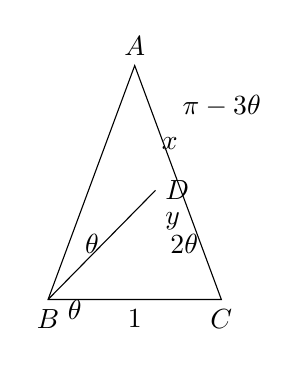
\begin{tikzpicture}[scale=2.2, >=stealth]
  \coordinate (B) at (0,0);
  \coordinate (C) at (1,0);
  \coordinate (A) at (0.5,1.35);
  \coordinate (D) at (0.62,0.63);
  \draw (B) -- (A) -- (C) -- cycle;
  \draw (B) -- (D);
  \node[below] at (B) {$B$};
  \node[below] at (C) {$C$};
  \node[above] at (A) {$A$};
  \node[right] at (D) {$D$};
  \node[below left] at (0.25,0.05) {$\theta$};
  \node[below] at (0.5,0) {$1$};
  \node[left] at (0.35,0.32) {$\theta$};
  \node[right] at (0.65,0.32) {$2\theta$};
  \node[right] at (0.6,0.9) {$x$};
  \node[right] at (0.62,0.45) {$y$};
  \node[above right] at (0.72,1.0) {$\pi-3\theta$};
\end{tikzpicture}
\end{center}

$\triangle BCD$ に正弦定理を用いて，
\[
\frac{x}{\sin2\theta}=\frac{1}{\sin(\pi-3\theta)}=\frac{1}{\sin3\theta} \quad\therefore\ x=\frac{\sin2\theta}{\sin3\theta} \quad \cdots \text{②}
\]
以下 $S=\sin\theta,\ C=\cos\theta$ とする。$\sin2\theta=2SC,\ \sin3\theta=3S-4S^3$ より，②から
\[
x=\frac{2SC}{3S-4S^3}=\frac{2C}{3-4S^2}=\frac{2C}{4C^2-1}
\]
これは $C$ の単調減少関数であり，①とあわせて，
\[
\frac23<x<\sqrt2 \quad \left(\because\ \frac{2C}{4C^2-1}\xrightarrow{C\to\frac{\sqrt2}{2}+0}\sqrt2,\quad \frac{2C}{4C^2-1}\xrightarrow{C\to1-0}\frac23\right)
\]
\end{proof}

\newpage

\section*{第3問}

\begin{proof}[解]
$(t,e^t)$ における接線 $\ell_t$ は，$(e^x)'=e^x$ より，
\[
\ell_t: y=e^t(x-t)+e^t \quad \cdots \text{①}
\]
である。これが $(a,b)$ を通る時，
\[
b=e^t(a-t)+e^t\equiv f(t) \quad \cdots \text{②}
\]
$y=e^x$ では，接点が異なれば接線が異なるので，②をみたす $t$ の数が $(a,b)$ から引きうる接線の数に等しい。
\[
f'(t)=e^t(a+1-t-1)=e^t(a-t)
\]
から，下表をうる。
\begin{center}
\begin{tabular}{c|ccc}
$t$ & & $a$ & \\
\hline
$f'$ & $+$ & $0$ & $-$ \\
\hline
$f$ & $\nearrow$ & $e^a$ & $\searrow$
\end{tabular}
\end{center}
したがって，$f(t)\to-\infty\ (t\to+\infty)$，$f(t)\to0\ (t\to-\infty)$ から，$y=f(t)$ のグラフは右上図のようになる。したがって，$a$ を固定した時，②は $y=b$，$y=f(t)$ のグラフの交点で与えられるので

\begin{center}
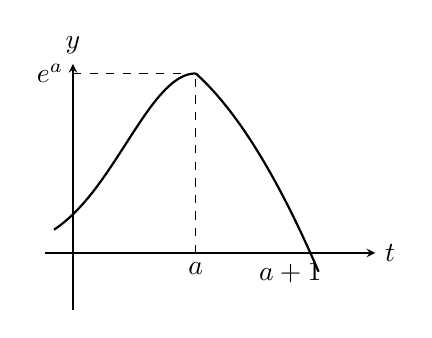
\begin{tikzpicture}[scale=1.2, >=stealth]
  \draw[->] (-0.3,0) -- (3.2,0) node[right] {$t$};
  \draw[->] (0,-0.6) -- (0,2) node[above] {$y$};
  \draw[domain=-0.2:1.3, smooth, thick] plot (\x, {1.9*exp(-((\x-1.3)^2)/1.1)});
  \draw[domain=1.3:2.6, smooth, thick] plot (\x, {1.9-0.9*(\x-1.3)-0.55*(\x-1.3)^2});
  \draw[dashed] (1.3,0) -- (1.3,1.9);
  \draw[dashed] (0,1.9) -- (1.3,1.9);
  \node[left] at (0,1.9) {$e^a$};
  \node[below] at (1.3,0) {$a$};
  \node[below] at (2.3,0) {$a+1$};
\end{tikzpicture}
\end{center}

\[
\begin{cases}
b\le0\ \text{の時，解は}1\text{つ} \\
0<b<e^a\ \text{の時，}2\text{つ} \\
b=e^a\ \text{の時，}1\text{つ} \\
b>e^a\ \text{の時，}0\text{個}
\end{cases}
\]
となる。$a$ の固定を解除して，
\[
\begin{cases}
b\le0\ \text{または}\ b=e^a\ \text{の時}\quad 1\text{個} \\
0<b<e^a\ \text{の時}\quad 2\text{個} \\
b>e^a\ \text{の時}\quad 0\text{個}
\end{cases}
\]
\end{proof}

\newpage

\section*{第4問}

\begin{proof}[解]
$f_n(x)=x^n\sin^nx$ とおく。さらに，$P(x)=f_1(x)$ とする。はじめに(2)を証明する。

以下，$P(x)=P,\ \sin x=S,\ \cos x=C$ などと書く。
\[
S_{n+2}+S_n>2S_{n+1}
\]
\[
\iff \int_0^{\pi/2}P^n(P^2+1)dx>2\int_0^{\pi/2}P^{n+1}dx
\]
\[
\iff \int_0^{\pi/2}P^n(P-1)^2dx>0 \quad \cdots \text{①}
\]
であり，$[0,\pi/2]$ では $0\le P,\ 0\le(P-1)^2$ だから，
\[
0\le P^n(P-1)^2
\]
$[0,\pi/2]$ で積分し，常には等号が成立しないことから，
\[
0<\int_0^{\pi/2}P^n(P-1)^2dx \quad \cdots \text{②}
\]
①，②から(2)が示された。以下(1)，(3)を示す。

ここで $S_1,\ S_2$ を計算する。
\[
S_1=\int_0^{\pi/2}Pdx=\left[-xC+S\right]_0^{\pi/2}=1
\]
\[
S_2=\int_0^{\pi/2}f_2(x)dx=\int_0^{\pi/2}x^2\cdot\frac{1-\cos2x}{2}dx
\]
\[
=\frac12\left[\frac13x^3\right]_0^{\pi/2}-\frac12\left[\frac12x^2\sin2x+\frac14\cdot2x\cos2x-\frac18\cdot2\sin2x\right]_0^{\pi/2}
\]
\[
=\frac16\left(\frac{\pi}{2}\right)^3-\frac12\cdot\frac14\cdot2\cdot\left(-\frac{\pi}{2}\right)=\frac{\pi^3}{48}+\frac{\pi}{8}
\]
であり，$\pi>3.14$ から
\[
S_2>\frac{\pi}{8}\left(\frac{3.14^2}{6}+1\right)>\frac{2.64}{8}\cdot3.14=\frac{8.2896}{8}>1=S_1
\]
\[
\therefore\ S_2>S_1 \quad \text{(1)}
\]
となる。したがって，(2)の不等式をくり返し用いて，
\[
S_{n+1}-S_n>S_n-S_{n-1}>\cdots>S_2-S_1>0 \quad\therefore\ S_{n+1}>S_n
\]
だから，$\{S_n\}$ は単調増加で，$m<n$ ならば $S_m<S_n$ となる。 \text{(3)}
\end{proof}

\end{document}
